%%==========================
%% chapter01.tex for SJTU Master Thesis
%% based on CASthesis
%% modified by wei.jianwen@gmail.com
%% version: 0.3a
%% Encoding: UTF-8
%% last update: Dec 5th, 2010
%%==================================================

%\bibliographystyle{sjtu2} %[此处用于每章都生产参考文献]

% 第四章的布局:
% 整体介绍,附图 1000
% 分块方法,简单分块,滑动块分块?1000
% 对分块预处理,一些复杂的方法,以及缺点 2000
% 预处理完进行FFT变换,分析理论 2000
% 对输出的结果与库中的值做余弦定理,提出\epislon参数 2000
% 加入spark以后算法的架构 2000

\chapter{基于FFT的文件去重算法}
\label{chap:algo}

\section{背景介绍}
\label{sec:back}

在第二章中,已经详细介绍了当今互联网大数据环境下的各种文件去重的核心算法,每一小节介绍算法分别改进和优化了前一小节中的算法并且在效率上有着显著的提升。

这些算法的主要思想是,先将文件分块,作为算法下一步的输入,分块的大小由系统的设定而决定,一般取值为使系统效率最高的那个值,分块的目的是为了更方面下一阶段的处理;接着共同的一步是对文件块进行哈希计算,比如SHA1的哈希值,需要注意的是,MD5也是一个比较好的方案,但是在一般的场景下用SHA1来代替MD5,一个最重要的原因是MD5已经被证明可以进行碰撞攻击。也就是说,攻击者可以产生两个应用程序,内容不一样,但是哈希值完全一样;将输出的SHA1哈希值与服务器上已经保存的哈希值做比较,若有发现符合,则说明这个文件块在服务器上已经有了一份拷贝,需要再次上传和存储;若没有发现符合,则认为这是一份新的文件块,客户端需要上传这份文件块。

在上述的通用算法中,一个很重要的一点是,只能检测两个完全相同的文件是否相同,如果一个文件的任意字节被改动,这两个文件即被视为不相同,即这是一个“零一”问题,要么相同要么不相同,没有中间的可能性。但是一个拥有这种中间可能性的检测算法在某些场景下是非常被需要的,比如若两个文件的文件内容的相似度达到95\%及以上的时候,这两个文件即可被视为相同的文件。一个典型的应用场景是一个新闻报导系统,在这个系统中规定相同内容的报导不能被同时报导两次,即若两条新闻都是关于X和Y关系的主题,系统应该检测出第二条新闻与前一条新闻相似并且予以警告,这个相似度系数可以按照系统的需求而调节,比如某些情况下完全不同的报导才是不一样的报导,这个时候相似度就是100\%,而某些情况下只要90\%内容相同则是相同的报导,本文提出的基于FFT的文件去重算法就是在这样的背景下提出的,这个算法中,有一个系统参数$\epsilon$,可以动态地调节系统对相似度的需求,有很大的灵活性。基于FFT的去重算法的其它部分(分块的选择,分块预处理,FFT变换,对输出进行处理和比较)将在下面的几个小节中一一介绍。

\begin{figure}[!hbp]
%\centering
    \begin{minipage}[b]{0.6\textwidth}
    \captionstyle{\centering}
    \centering
    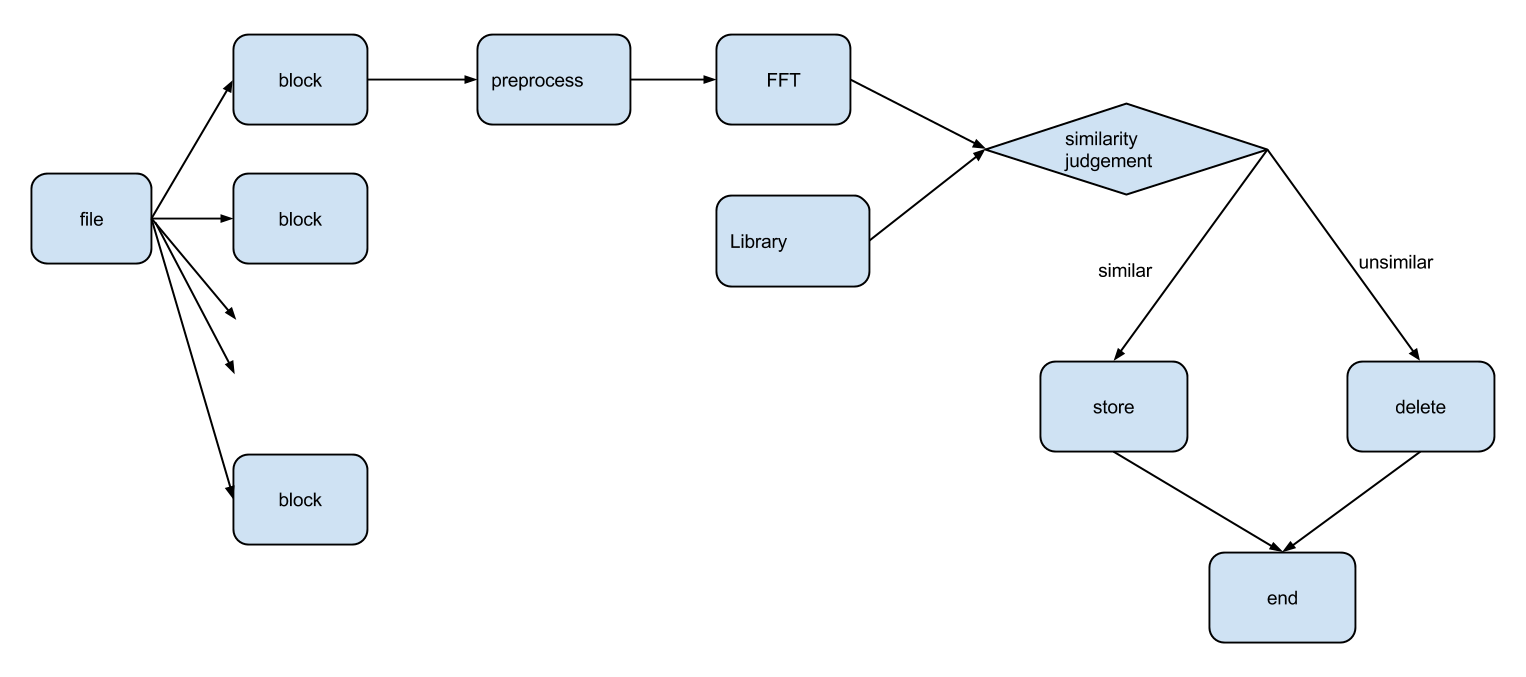
\includegraphics[origin=br,width=18cm]{chap4/archti.png}
    \bicaption[fig:archti]{算法架构}{基于FFT的文件去重算法架构.}{Fig}{Archtecture.}
    \end{minipage}     
\end{figure}

在图\ref{fig:archti}中,简单得描述了这个算法的简要步骤,首先,基于一些方法将一个大文件分成若干个文件块,这个文件块的输入将作为预处理的输出,预处理的输出将作为FFT的输入,FFT的输出是一个N维的向量,此时这个向量就代表了这个文件块,称为文件块的特征向量,与服务器端的库文件进行相似度的测试,此时需要依赖系统参数$\epsilon$,若相似,则不存储;若不相似,则存储,算法结束。本章节将详细介绍每一步骤的算法和设计理念。

\section{分块方法}
\label{sec:choice}

在第二章我们简单地提到过,若使用简单分块的方法,即对任意一个文件按照固定长度的切分成一个个文件块的方法,会遭受到插入问题(insertion problem)和删除问题(deletion problem)的影响导致去重性能急剧下降。简单来说,若采用简单分块的方法,那么边界是由预定义的分块大小决定的,此时如果任意插入或者删除一个字符,那么在这个分块之后的所有分块的内容都会向后或者向前偏移一个字符,导致了这个分块以后的所有分块都不相同,造成的结果是,即使后面的文件块毛无变化,但服务器上还是会存储多分冗余的拷贝。解决这个问题的一个方案是,不采用基于文件块大小作为块划分边界的依据,而是采用另外一种方法,即先定义一个滑动窗口,若文件的某一个滑动窗口满足一定事先约定的条件,那么这个滑动窗口对应的最后一个字节才是这个分块的最后一次字节。采用这种分块方法的好处的是,若随便插入或删除一个字符,那么只会影响当前块和之后的一个块,而其它块均不受影响,大大提高了存储的效率,此时的文件分块不再是以内容长度作为边界的依据值,还是根据内容。在本文基于FFT的文件去重算法中,我们采用简单分块的方式而不是基于滑动窗口的方法,理由主要是以下几点:

\begin{enumerate}
\item 保证了模型的简易性,将重点放在了FFT,余弦定理和系统参数$\epsilon$上
\item 在仿真阶段我们实现系统的主要框架,用简单分块大大简化了原形的实现
\item 本算法的重点并不是分块方法,可以由专门的论文来详细讨论
\end{enumerate}

事实上,若将此算法应用在工业界的实际使用中,那么考虑到存储的效率等等因素,一般还是会采用基于滑动窗口的分块方式,在之后的所有讨论中,将默认采用的时简单分块的大小,即直接将文件通过块的大小分成若干份,在服务器上的所有数据都是以块为单位,一个文件由若干个块组成。

\section{分块预处理}
\label{sec:proproc}

在本章中,将详细讲解分块预处理的必要性以及具体方法和步骤,我们将讨论一个现有的分块预处理的方法,分析这个方法的优缺点,并提出一种简单高效的分块方法。

\subsection{为什么要预处理}
\label{sec:why}

在\ref{fig:archti}中,我们可以看到,当文件分块以后,要经过一个预处理的过程,这一步是十分必要的,它的作用是将不同形式的输出和输入能够非常好地连接在一起,比如复数形式的FFT的输入是一个N维的复数向量,而一个分块是一个文件,它是一个个字节组成的数据,怎么接近无缝地连接这两个模块是十分重要的,在本文中,将详细讨论这个过程。

\subsection{预处理的方法}
\label{sec:appro}

在一个现有研究中,利用了离散傅里叶变换来解决网页去重,在这个算法中,把每个字符都映射成一个字符,那么每篇网页就可以表示成一个离散的序列$y(i)$,重复的网页应该具有相似的序列,对该序列进行离散傅里叶变换就可以得到傅里叶系数$a_n$和$b_n$,然后通过某种方法比较两个网页文件的傅里叶系数的前几项就可以大致比较出两个网页的相似度。在这篇研究中,预处理的方法主要是将一个字符映射到该字符对应的语义数值。

一个比较合适的字符到语义数值的转化应该满足,语义上相似的字符值对应的语义值应该相近,语义上不相似的字符值对应的语义值应该相差较大。该方法采用了如下方法作为计算每个字符的语义值的方法:以大量互联网上的文本素材作为基础,统计这些文本材料中字符和字符出现的关系,假设不同的字符数为N,那么统计的结果将是一个$N \times N$矩阵,其中$R(i, j)$的值定义为字符i和字符j相邻出现的次数除以字符i在文本素材中出现的总次数,若$i==j$,则这个值被定义为1,于是字符i的语义值就可以由N维向量$R(i)$来表示,但$R(i)$是一个向量,我们需要的是一个数值,也就是说需要对这个N维向量进行降维的操作,在该研究中采用K-L变换(Karhunen-Loeve)\upcite{vranic2001tools}的方法对$R(i)$降维,它是一种建立在统计特性基础上的一种转化,目的是将数据做转化,使得转化后数据的相关性最小。基于语义的预处理方法的优点是,这样的预处理方法比较新颖,并且是基于语义的,基于语义的一个最大的好处就是能够非常接近真实地反映原来数据之间的关系,并且能按照这样的关系模拟出一个具体的数值来代表这种关系,在某些基于语义的去重的场景下,这样的算法将非常合适。

实际上,对于互联网上的大数据而言,使用基于语义的预处理意义并不是特别大。首先,通常意义下的去重算法只关心两个文件严格意义上是否相同,即任意字符就代表文件的一个标志位,若这个字符不相同,则两个文件则不相同,而不在意这个字符与下一个字符之间的关系;其次,在上述的描述中我们需要实现构建一个$N \times N$的矩阵,这个矩阵是基于互联网上大量的文本素材所构建的,但是在实际中,这些素材的来源将很大程度上决定了这个$N \times N$矩阵的性质,需要严格保证这些素材的随机性,不仅如此,N将会是一个非常大的数字,表的一部分可能存在磁盘中,导致了一次读取表的操作都可能引起一次潜在的磁盘读取,对于高时效性高性能的大数据计算,这样的延时显然是不允许的。综上,基于语义的算法有很多不足之处,本文将提出一种简易的,可实现的同时具有保真性的预处理算法。

由分析可知,字符和字符之间的语义关系是不会影响两个文件之间相似度的判定,于是在本文中,将直接将文件的每一个字节看作是一个个离散的点,每个点取值范围为0至255,作为输入复数组中每一个复数的实数部分,即若一个1MB的文件经过预处理,则输出的是一个1*1024*1024维的复数向量,其中实部$real(i)=$第i字节对应的值,虚部$imag(i)=0$。这么做的好处有以下几点:

\begin{enumerate}
\item 完全脱离了语义的束缚,把着重点放在了每个字节上;
\item 从抽象角度上,更容易理解怎么把一个文件映射成一个离散的信号,以此作为FFT的输入;
\item 提高设计的简单性,实现的可行性。在仿真阶段,如果采用基于语义的预处理方法,将大大增加仿真的复杂度和难度,首先文本样本的选择是第一个问题,其次对于有些小型机器内存不一定能完全放下,这些在上面已讨论过。
\end{enumerate}

在下一小节说,将详细说明对变换后的文件使用傅里叶变换的意义和具体算法。

\section{对文本进行FFT变换的意义}
\label{sec:ffttr}

\subsection{文本作为离散的点}
从本质上来说,傅里叶变换不仅仅是一个数学工具,更是一种看待事物的一种思维方式,从时域上来讲,一切事物都在变化,换一个角度,若从频域上来讲,好像一切都是事先约定好的,有规律可循的,静止的。本章节将从抽象的角度来阐明怎么把FFT应用在文件去重这个领域上。

对于计算机而言,DFT是唯一能应用的一种傅里叶变换的变体,在数学的推导中,函数可以是连续的,所以有连续傅里叶变换和离散傅里叶变换,但计算机无法处理连续的信号,它只能对连续的信号进行采样,然后处理这些有间隔的离散的点。一个比较常用的例子是,音频信号在时域中显然是连续的,但计算机在记录音频并做处理的时候需要先对音频信号进行采样,两个样本之间会经历一个很小很小的时间$\Delta t$,于是整个音频的信号就可以变成时域上若干离散的点,从而可以进行下一步的处理。

理解傅里叶变换对输入转化的抽象意义是本文的一个难点,为了帮助读者理解对文本进行FFT变换的意义,将先举一个音乐的例子。在没有学习过乐器的人的理解中,音乐就是随时间变化的震动;而在一些乐器玩家的理解中,音乐是那些在乐谱上的音符。前者的理解是音乐在时域中的样子,而后者的理解是音乐在频域中的样子。在时域中,我们看到音乐随着琴键的上下按动而发出声音;在频域中,音乐是一些永恒的音符。对于任何一首乐曲,都可以通过不同琴键在不同的时间的敲击组成,其实本质上说的就是,任何周期函数,都可以看作是不同振幅不同频率不同相位的正弦波的叠加。

然后我们再来看离散的傅里叶变换,DFT的正向变换公式如下:$$X(k)=\frac{1}{N}\sum_{n=0}^{N-1}x(n)(\cos(\frac{2\pi kn}{N}) - j\sin(\frac{2\pi kn}{N}))$$可以很容易地看出,在频域上每一个点k对应的幅度值,都是由时域上所有点的加权和,而这个权重每个点都不一样,将欧拉等式应用于上式,我们可以得到$$X(k)=\frac{1}{N}\sum_{n=0}^{N-1}x(n)e^{-j2\pi kn/N}$$本文的一个难点是要理解将一个个分块的文件看成是一堆离散的信号,这是一种看待问题方式的创新和转变,也是傅里叶变换能够应用在很多领域(比如物理学、结构动力学、密码学等等)的一个重要原因,万事万物若从抽象的角度来看待均由一系列离散的点构成。我们将文件块经过预处理算法变成向量以后,对这个向量进行快速傅里叶变换,输出的这个N维向量可以看成是这个文件块的另外一种表达方式。在输出的N维向量中,每一个频率上的幅度值都由原来离散信号的所有点共同决定。

\subsection{FFT的必要性}

在上面的讨论中,我们看到,FFT的输入是一个N维的向量,输出也是一个N维的向量,那么为什么一定要经过FFT,直接用FFT的输入放到算法下一步的输入,即省去FFT这一步可以吗?答案是否定的。在下一节中,要解释这个问题需要先理解下一小节的内容,即我们是怎么处理和比较N维向量的,这是整个算法的最后的最后一步,两个N维向量若相似则说明找到重复,若不相似,说明这是一份新的文件块,服务器将存储文件块。在我们的算法中将定义两个变量CHECK\_UP和CHECK\_DOWN,若不进行FFT的变换,则会产生任意一个改变字符的权重全部加在了当前字符上,而我们希望这个字符的变化可以对整体的相似度的变化有影响,FFT非常好地完成了这项工作,每一个频率上的幅度都是由原来时域上的点加权得出。

\section{N维向量相似度的比较}
\label{sec:Nsimi}

\subsection{余弦定理的局限}

在现有技术中,比较N维向量相似度的一个主要的算法是余弦定理,这个算法非常容易理解,余弦定理算的时两个N维向量之间的夹角,若两个向量在坐标轴上靠得非常近,即之间的夹角非常小,那么我们就可以认为这两个向量是相似的向量。这个技术方法曾经被用在谷歌的新闻分类中,当时这个方法在分类领域的应用是一个非常大的创新点。本文算法设计的时候一开始也是将余弦定理为算法的输出比较,但是在写代码做实验的时候发现,余弦定理中有一个非常大的局限性,并且FFT的输出向量正好落在了这个局限性里头。

在上面的讨论中,我们谈到,在频域上任何一个点的幅度值都是由在时域上所有点加权的结果,那么有的点权重大有的点权重小,在加上文件本身对应的离散值的取值范围是0至255,同一个文件块的离散信号可能相差较大,这就导致了经过FFT变换以后维度和维度之间的数量级会相差特别大,下面的这幅图是应用基于FFT和余弦定理的算法的输出,其中$i$表示第几个点,$value$表示经过变换FFT变换以后的值。

\begin{lstlisting}[language={C}, caption={基于余弦定理检测相似度的结果}]
file "data_16_1" size is 16!
i = 0, value = 1162084.000000
i = 1, value = 31571.293828
i = 2, value = 9547.236365
i = 3, value = 4196.636560
i = 4, value = 1300.000000
i = 5, value = 12953.890439
i = 6, value = 10972.763635
i = 7, value = 8478.179173
i = 8, value = 20164.000000
i = 9, value = 8478.179173
i = 10, value = 10972.763635
i = 11, value = 12953.890439
i = 12, value = 1300.000000
i = 13, value = 4196.636560
i = 14, value = 9547.236365
i = 15, value = 31571.293828

file "data_16_2" size is 16!
i = 0, value = 1060900.000000
i = 1, value = 33937.760974
i = 2, value = 21162.751504
i = 3, value = 4277.091378
i = 4, value = 3412.000000
i = 5, value = 9801.435621
i = 6, value = 3581.248496
i = 7, value = 3039.712027
i = 8, value = 8836.000000
i = 9, value = 3039.712027
i = 10, value = 3581.248496
i = 11, value = 9801.435621
i = 12, value = 3412.000000
i = 13, value = 4277.091378
i = 14, value = 21162.751504
i = 15, value = 33937.760974
cos = 0.999735
\end{lstlisting}

在这个实验中,我们的两个文件分别是16字节,是两个完全不相似的文件。可以很明显看到第0个点的值的数量级远远大于别的维度值的数量级,导致的结果就是这一维的作用可能使别的维度效果非常非常小,于是这两个16维向量的夹角将非常地近,最后一行是两个向量的余弦值,可以看到夹角几乎为零。即对于两个不相似的文件,输出的结果是相似。

\subsection{一种新的方法}

事实证明,基于余弦定理的算法设计是有问题的,此时我们有两个选择:第一,改进现有的余弦算法,目的是让所有维度的值都在同意数量级内,因为不同维度的数据关系本来就不大,很难找到一种方法达到这样的目的;第二,设计一种新的算法,达到同样的目的。本文将采取第二种做法,设计一种新的做法来计算两个N维向量的相似度。算法的的代码如下:

\begin{lstlisting}[language={C}, caption={检测两个N维向量的相似度}]
int calc_simi(vector<double> &da, vector<double> &db, double &result)
{
    if (da.size() != db.size())
    {
        fprintf(stderr, "two vector size must be equal.\n");
        return THES_FAIL;
    }

    size_t vsize = da.size();
    int count = 0;
    for(size_t i=0; i < vsize; ++i)
    {
        double qt = da[i] / db[i];

        if (qt > CHECK_UP || qt < CHECK_DOWN)
            continue;

        count++;
    }
    
    result = double(count) / vsize;
    return THES_SUCC;
}
\end{lstlisting}
算法的输入是两个向量,分别放在两个vector里面,首先判断两个向量的长度是否一致,如果不一致,那么就错误,程序退出,文件在分块的时候就保证每个向量长度都是一致的,然后遍历这N维向量,定义一个上界CHECK\_UP和下界CHECK\_DOWN(这两个值可以用户自己配置以达到最佳效果),如果$da[i]$与$db[i]$的比值大于CHECK\_UP或者比值小于CHECK\_DOWN,那么就说明第i维度的两个值相差太远,视为无效维;否则,视为第i维度对整体的相似度有贡献,表现为将count加一,循环这个过程,直到全部处理完这两个N维向量,最后将count值除以向量的长度返回,这个值被我们定义为两个N维向量的相似度。

\subsection{可调节的相似度算法}

在这一节中,我们将定义一个系统参数$\epsilon$,取值范围$[0,1]$,来满足不同情况下对相似度的要求。我们定义,若两个文件的相似度大于$1-\epsilon$,那么这两个文件就是相同的文件。所以,这个值越大,就对相似性的要求越高。

从这个定义我们可以容易地得出,在两个极端的情况下,当$\epsilon$为0时,则只要任何一个字节不同,就被视为不同的文件;而当$\epsilon$为1时,则任何两个文件都会被视为相同的文件。所以这个参数的提出大大提高的算法应用场景的适应度,在传统的文件去重环境中,我们只要将这个系统参数设定为$0$即可。

这个系统参数的提出是个较新的做法,据我们有限的知识,以前还未在这个领域使用过类似的可配置的参数来调节不同场景对不同相似度的要求,这个参数具体影响的效果是使得查全率(正确去重数量 / 存在的重复)提高了,而使准确率(正确去重数量 / 存在的重复)下降了,所以正确地调节此值就非常重要。

\section{基于spark的算法设计}
\label{sec:spark}

在当下的大数据的环境下,spark已经受到了业界的一致好评,基于MapReduce的分布式计算方法也使得spark非常类似于Hadoop,保留的Hadoop优点的情况下,却又比Hadoop的通用性更加,迭代的运算效率更高,容错能力更强,所以在未来spark的发展前景可能会超越Hadoop,称为更通用的并行计算框架。在\cite{zaharia2012resilient}中,描述了RDD通用的架构,RDD是spark的基本构造模块,类似于分布式的不可变集。这些定义的操作如map或foreach,能很容易地并行处理;join运算,需要两个RDDs和一个共同建条目;规约的时候,通过用户指定基于键的函数来聚合条目。RDD从磁盘读取,然后为了提高之后的处理速度将数据都保存在内存中,也可以通过别的途径进行缓存,那样就可以不用每次都去读取他们,仅仅是这些基于提升磁盘速度的优化就比Hadoop块快了许多。当然,spark可能不会适应所有的场景,类似只更改很少条目的操作就不合适。原则上,就算只对一个条目修改,也必须对整个数据集备份。

在本章中,将设计一个并行算法,来执行我们的并行文件操作。在文件去重的领域,并行化是明显的趋势所在,除了第二章所提到的全文件检测算法以外,其它的算法均涉及到了文件分块的操作,所以这里有很多并行的工作可以做。

\begin{figure}[!h]
%\centering
    \begin{minipage}[b]{1\textwidth}
    \captionstyle{\centering}
    \centering
    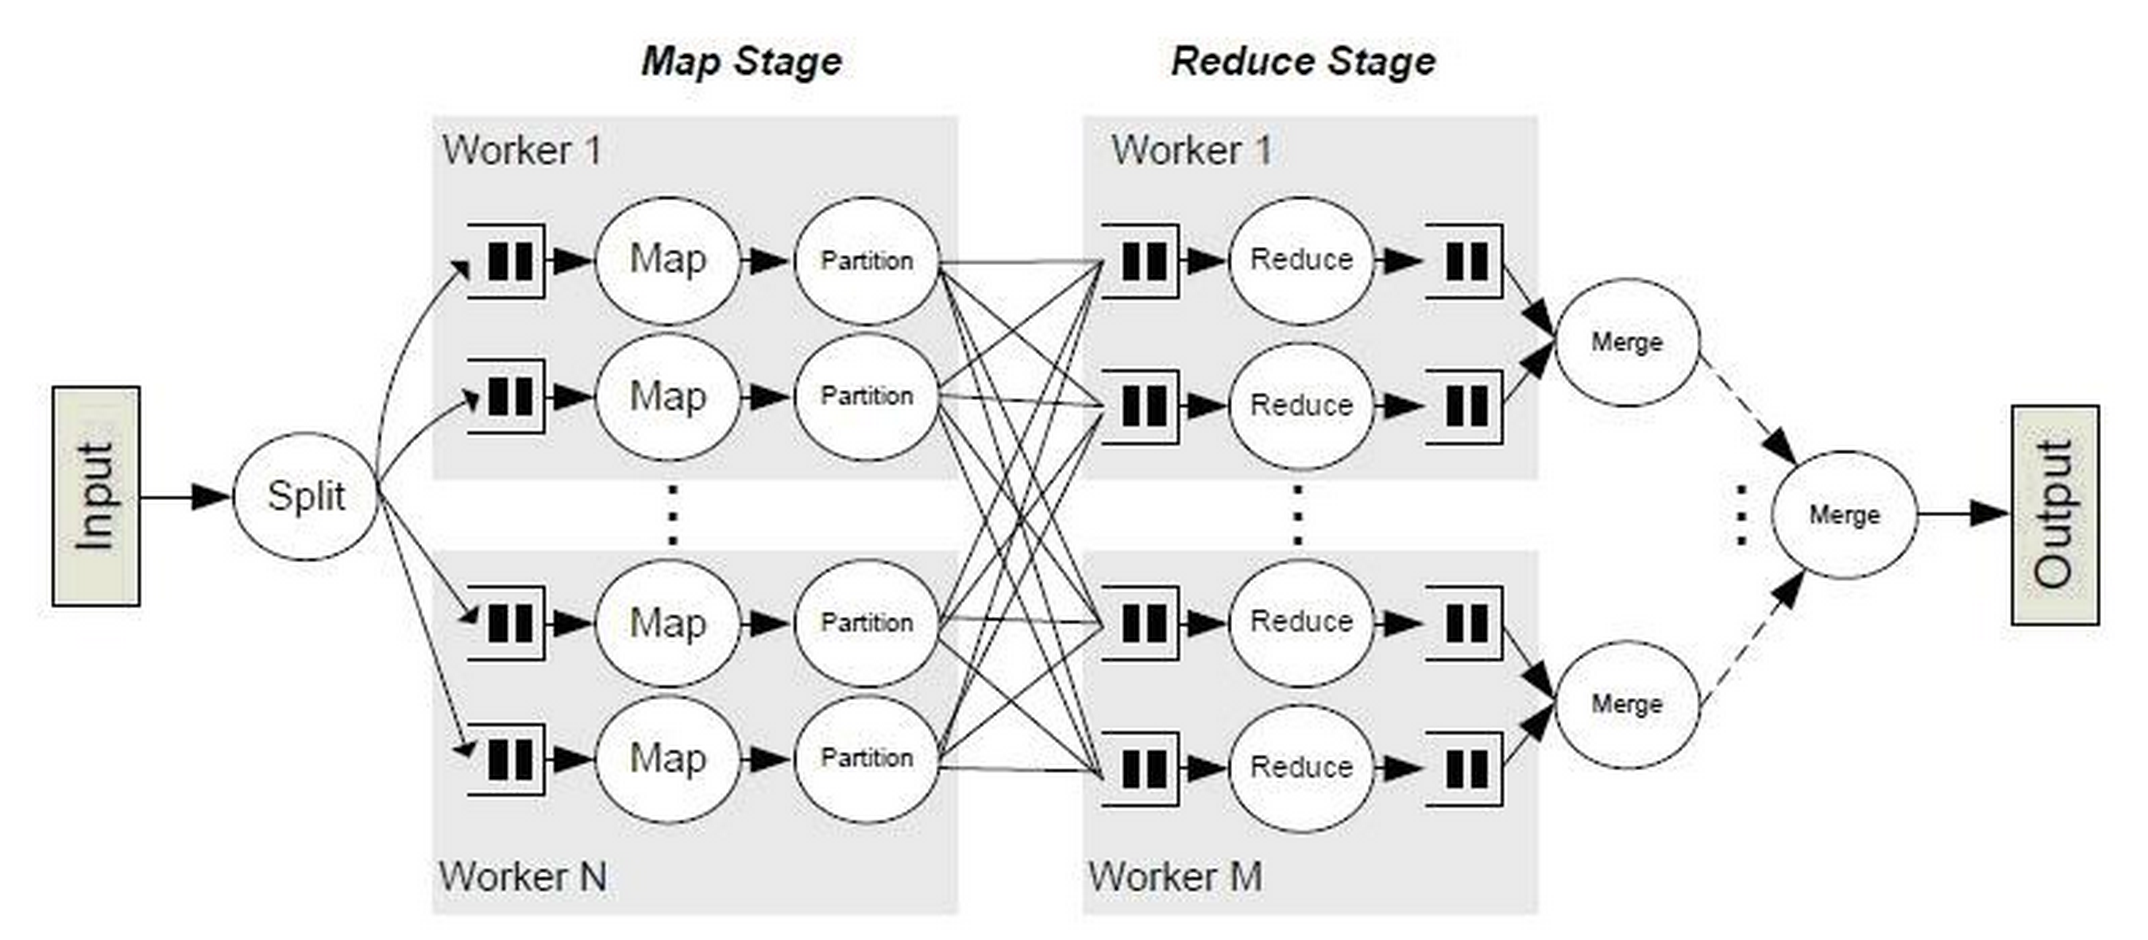
\includegraphics[origin=br,width=16cm]{chap4/sparkmapreduce.png}
    \bicaption[fig:sparkmr]{spark MapReduce框架}{spark MapReduce框架}{Fig}{spark MapRedeuce Framework.}
    \end{minipage}     
\end{figure}

在图\ref{fig:sparkmr}中,显示了spark Map Reduce的通用框架图,首先将输入进行split操作,分成一块块可以并行操作的小块,之后进行map操作,输出进行partition分配到各自的reduce节点,reduce操作完了以后进行merge的操作,最后将结果输出。这个框架下最经典的一个例子是wordcount,计算一篇文章中每个单词出现的次数,用这个并行框架可以完美的结果,我们也将应用这个经典的框架在基于FFT的文件去重算法上,达到加速的目的。

用户的文件是一个大文件,我们将用户的文件拆分成小块,例如8MB或者16MB,这个值将由具体系统确定,那么在后台整个文件就可以由一个结构体来表示,结构体的一个成员是一个指向分块的指针数组,还原文件的时候只要遍历这个数组一次输出文件块的内容即可。下面我们将依次介绍Map Reduce框架中具体的细节:

\begin{enumerate}
    \item Split

        Split操作对应的是文件的分块操作,如果系统的文件块大小设定为16MB,那么用户输入一个1G文件时,这个文件将被分成64个文件块,于是系统将不再看到“大文件”这个概念,系统将看到的是64个固定文件块作为输入。将分成的这N个文件块分别塞入workers的队列中,等待worker读取进行下一步的Map操作。
    \item Map

        Map的输入是已经分好块的文件块,具体要做的是先对文件块做事先约定好的预处理,即把整个文件的字节值作为离散的点。然后进行快速傅里叶变换,此时的输出是一个N维的向量,这里的N等于文件块的大小。

    \item Partition

        Partition这一步将前面Map输出的N维向量分配到各个reduce节点,具体的分配方法有非常多,可参考现有的一些做法,一种比较普遍的方法是先讲N维向量降维成一维,然后哈希后取模作为reduce worker的序号。
    
    \item Reduce

        在reduce这一步与服务器上已有的文件进行比较,若发现满足任何在服务器上已有的快与这个块的相似度大于了$1-\epsilon$,那么就说明发现了重复的文件,那么保存一个指向相同文件块的指针即可;若与所有文件块的相似度都小于$1-\epsilon$,那么为这个文件块创建一片存储区域,服务器将存储这个文件块,并将指针指向这个新的文件块。

    \item Merge

        Merge的过程即是创建代表这个文件的结构体的过程,这个结构体里保存一个指针数组,这个数组的值由上一步Reduce产生,或指向新的文件块或指向旧的文件块。至此,一次上传文件的操作就完成了。
\end{enumerate}

在上述描述中,我们可以看到,若一个文件全部的文件块都是重复的,那么服务器上不用对存储这个文件做任何实质性的操作,只需要保存这个文件的元数据,即表示这个文件的结构体,也是会占用一部分系统资源,但是相比文件本身的大小,这个值可以忽略不计。

\section{小结}
\label{sec:conclusion}

在本章中,提出了基于FFT文件去重算法,首先介绍了算法的主要思想和具体框架,接着讨论了一些分块方法的优缺点和我们采用的方法以及选取的原因,我们又讨论了分块预处理这一过程,阐述了为什么要进行预处理以及一些现有的预处理方法和我们采用的方法;然后我们详细说明了对文本进行FFT变换的意义,包括将文本作为离散的点这种比较创新的思维方式,之后我们又讨论了进行FFT变换的必要性;我们又讨论了了两个N维向量相似度的比较算法,提出了余弦定理的局限性的同时提出了一种可调节系统参数$\eplison$的方法,最后,我们还设计了基于spark内存计算并行框架的算法实现。在下一章中,主要讨论我们实现的一个原形系统,从框架上实现了我们本文所提到的算法,并用一种用户友好的方式展现出来。
